%preamble
\documentclass[letterpaper]{article}
\synctex=1
\usepackage{graphicx}
\graphicspath{ {images/} }

\usepackage{lipsum}
\usepackage{float}

\usepackage{amssymb}

\usepackage{siunitx}

\usepackage{multirow}
% for merging table cells I think

\usepackage{tabularx}
\renewcommand\tabularxcolumn[1]{m{#1}}% for vertical centering text in X column

% allows for linewrap within cells
\newcolumntype{Y}{>{\centering\arraybackslash}X}

\usepackage{todonotes}
\usepackage{hyperref}

\usepackage{pdfpages} % for attaching the table lol

%for plots
\usepackage{tikz}
\usepackage{pgfplots}
\pgfplotsset{width=8cm,compat=1.15}\usepgfplotslibrary{patchplots}
\title{ECE 322 \\
Lab Report 1}
\author{Arun Woosaree\\
XXXXXXX}
\begin{document}
\maketitle
\section{Introduction} The purpose of this lab was to serve as a practical
introduction to some more black box testing techniques. In this lab, the
testing methods introduced were the Extreme Point Combination (EPC), and the
Weak n x 1 strategy methods. We tested two programs written in Java using both
of these testing strategies. The first application, named Drone takes in three
arguments, and outputs either `Success!', `Failure', or an error message based
on whether the arguments are integers $\geq 0$, and their sum is less than
$k=100$. The second program, named RemoteCar takes in two arguments which
represent points on a Cartesian plane, and outputs either `Ok', `Out of range',
or an error message based on whether the point is on a circle of radius 1 about
the origin. The idea for EPC testing is to identify the input domain limits,
and produce all possible combinations of inputs with each of the input
variables taking on a minimum value, slightly under minimum, a maximum value,
and slightly over maximum value. One additional test case is added somewhere
within the valid subdomain to generate a total of $4^n + 1$ test cases, where
n is the dimension of inputs, or put more simply, the number of input
variables. With the weak n x 1 strategy, we attempt to find linear boundaries 
of the problem using domain analysis. $n$ points are selected on each linear
boundary, where $n$ is the number of input variables, and one additional point 
is chosen outside of each boundary. An additional point within the boundary is
chosen if the boundary is open, and if the boundary is instead closed an 
additional point outside the boundary is chosen. In the end, with the weak
n x 1 strategy, $b \times (n + 1)$ test cases are generated, where b is the 
number of linear boundaries, and n is the dimensionality, or the number of
inputs.

\section{Task 1 - Drone}
For task one in this lab, the Drone application was tested using both the
EPC method and the weak n x 1 strategy. Drone is a command-line program
written in java, which takes three inputs, $x_1$, $x_2$, and $x_3$.
If $x_1 + x_2 + x_3 \leq k$, where $k=100$, the program should output
`Success', and if not, it should output `Failure'. The three inputs 
must be integers $\geq 0$. 

\subsection{Sudomain plot}
The subdomain for this problem is illustrated below:
\begin{figure}[H]
	\centering
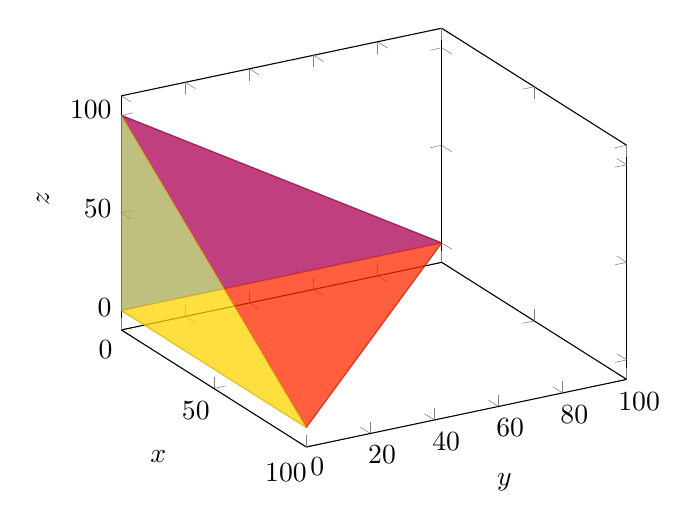
\begin{tikzpicture}
\begin{axis}[view/h=60,xlabel=$x$,ylabel=$y$,zlabel=$z$]
\addplot3 [
opacity=0.5,
table/row sep=\\,
patch,
patch type=polygon,
vertex count=3,
patch table with point meta={
% pt1 pt2 pt3 pt4 pt5 cdata
0 1 2 0\\
0 1 3 1\\
0 2 3 2\\
1 2 3 3\\
},
] table {
x y z\\
0 0 0 \\%0
0 0 100\\%1
0 100 0\\%2
100 0 0\\%3
};
% replicate the vertex list to show \coordindex:
%\addplot3 [only marks,
%nodes near coords=\coordindex,
%] table [row sep=\\] {
%0 2 0\\ 2 2 0\\ 0 1 3\\ 0 0 3\\
%1 0 3\\ 2 0 2\\ 2 0 0\\ 1 1 2\\
%};
\end{axis}
\end{tikzpicture}
\end{figure}
The full list of test cases, along with the inputs and expected versus actual outputs can be found in Appendix.
The test cases where the expected result does not match the actual result are highlighted in red.
From experience, these test failures could be due to the following:
\begin{itemize}
    \item numbers like $2^{512}$ are ridiculously big. It's likely that that the implementation was not designed to handle such large numbers.
    \item similarly, numbers like $2^{-512}$ are so small that the calculator interprets it as being the number 0
    \item entering nothing results in an output of 0. It's likely that a lone space is interpreted as a 0 by the calculator
    \item if there's a space between a number and the minus sign after it, the calculator outputs NaN. It could be that when parsing the input, the calculator may be interpreting it as two numbers with no operator in between, so it does not know what to do and returns an error (NaN)
    \item the calculator does not follow the correct order of operations.
          If there's a division and multiplication. (e.g. $80/4*5$),
          it appears to be doing the multiplication before the division,
          even though the multiplication should be done afterwards,
          since it is on the right hand side of the previous division operation.
    \item when multiple exponent (\textasciicircum) operators are used in between two operands,
          the result is always one, instead of showing an error. This might be because the right half is evaluated as 0 by the calculator,
          and anything to the power of 0 is 1.
    \item when the first operand is missing for $+$ the calculator seems to ignore it and treat it like a positive number. This is why the calculator says $2++++2=4$
    \item when the first operand is missing for $*$, $/$, or \textasciicircum, the calculator evaluates it as being equal to 0 instead of returning an error.
          % This becomes apparent in operations like $\textrm2$,  $2**2$, or $/2$
    \item with the exponent operator, the calculator tries to evaluate everything after the exponent.
          however, this violates the BEDMAS rule in cases where the exponent should be done before multiplication, division, addition, or subtraction.
          This results in errors like $2^1+1$ resulting in 4 instead of 3.
          This also compounds with the previous errors in some cases where an expression like $2^3 + 2^3$
          is incorrectly evaluated as $2^5$, since $3+2$ is evaluated first, which results in 
          \textasciicircum 3
          being evaluated as 1, and the expression is reduced to $2^{5}$, resulting in the incorrect response.
    \item when numbers are only separated by a space, the calculator concatenates the digits. i.e. 1 2 becomes 12, instead of showing an error.
          when these numbers are wrapped by brackets, the calculator still concatenates them instead of multiplying. e.g. (2)(2) becomes 22 instead of 4.
          However, multiplying negative numbers using brackets e.g. (2)(-2) instead of the * operator results in a NaN error.
    \item the calculator has some rounding issues, which result in a loss of precision in the answer. Adding numbers like $2.000001+2.000002$ result in a rounded
          answer instead of the exact answer.
\end{itemize}
% \todo{fix the table and highlightthe failed test case}

\section*{Part 2 - Partition Testing}
Task two of this lab involved partition-based testing of a triangle application.
The purpose of this application is to take 3 space separated positive integers,
each representing sides of a triangle, and the program is expected to tell the
user whether the triangle is a scalene, isosceles, or equilateral triangle.
The following equivalence classes were decided on for creating the test cases.
\subsection*{Triangle Equivalence Classes}


From these equivalence classes, the following test cases were created:

\subsection*{Test cases for valid inputs}
\begin{itemize}
    \item 3 3 3 covers (1, 2, 3, 4, 7, 8)
    \item 4 4 5 covers (1, 2, 3, 5, 7, 8)
    \item 6 7 8 covers (1, 2, 3, 6, 7, 8)
\end{itemize}

\subsection*{Test cases for invalid inputs}
\begin{itemize}
    \item 1 2 covers (9)
    \item 3 4 5 6 covers (10)
    \item 7 8 \qquad 9 covers (11)
    \item 8\_7\_6 covers (12)
    \item 1 $-2$ 3 covers (13)
    \item 5 0 4 covers (14)
    \item 3 2 0.1 covers (15)
    \item 2 2 4 covers (16)
    \item 3 4 9 covers (17)
    \item not pressing Enter covers (18)
\end{itemize}

The results of these test cases, including expected versus actual output can be found in Appendix.
Failed test cases are highlighted in red. There was one test case which failed. 

\begin{itemize}
    \item For the input where we have the case $a+b=c$,
    (2 2 4) in this case, the program tells us that it is a isosceles triangle instead of an invalid one.
    This is likely because the implementation checks validity by looking for $a+b>c$ instead of $a+b \geq c$.    
    Similarly, with the inputs (1 2 3), the program tells us that it is a scalene triangle instead of showing an error.
\end{itemize}

\section*{Conclusion}
In this lab, we were introduced to black-box testing. The techniques
learned were dirty testing, error guessing, and partition-based testing.
Dirty testing's strength seems to also be its weakness at the same time. That is,
the test cases written are only limited by the tester's creativity.
One disadvantage, however, is that one can generate a lot of extra test cases
that are arguably unnecessary. That is, there is the possibility of having multiple
tests which cover the same functionality of the program. This is a problem that
using the partition-based testing method addressed. While equivalence testing allowed us 
to write significantly fewer test cases,
it does not catch some unique cases. For example, if dirty testing was done instead,
one might have tried the test inputs $$1111111111\ 1111111111\ 1$$, which returns ERROR: Invalid triangle
instead of saying that it's an isosceles one. This error, and potentially others were not
caught using partition-based testing. What is interesting, though is that the one
test failure with inputs (2 2 4) for the Triangle program allowed for another error to be found, which is
the case where an input like (1 2 3) which should cause an error instead returns `Scalene'.
Overall, it would not be fair to say that
one testing method is universally better than the other, however, the tester would
need to use their judgement and experience to choose an appropriate testing method
for the software that they want to test.

\vfill
\appendix
%\section*{Appendix}

\includepdf[pages=-]{EPC-drone-table.pdf}
\includepdf[]{weaknx1-drone-table.pdf}

\includepdf[]{EPC-remotecar-table.pdf}
\includepdf[]{weaknx1-remotecar-table.pdf}

\end{document}
